\chapter{Learning with Gradient}

\section{Gradient Descent}

Gradient Descent is a general approach to find the minimum of a differentiable convex function $J(\Vec{z})$ where $J (\Vec{z}): \mathbb{R} \rightarrow \mathbb{R} $ moving in the direction of the negative gradient. The Gradient Descent algorithm works as follows:

randomly initialize: $\Vec{z}~^{(0)}$

for $t = 1, ..., T$

~~~~~ $\Vec{z}~^{(t+1)} = \Vec{z}~^{(t)} - \eta \nabla(J(\Vec{z}~^{(t)})) $

output: $ \Vec{z}~^{(T)} $

\begin{figure}[h]
    \centering
    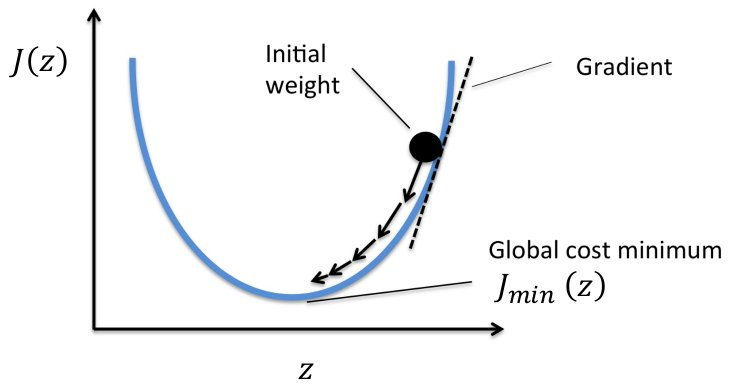
\includegraphics[width=10cm]{Images/gradient_descent.jpg}
    \caption{Gradient Descent algorithm update}
\end{figure}

where $\eta$ is the learning rate which indicates the size-step that we take at each update of the gradient.

\noindent The algorithm converges when the gradient is zero (or almost zero). Even though that in very simple cases we may be able to analytically solve $ \nabla J(\Vec{z}) = 0$ this is not the case for Deep Learning models. We have to keep in mind that in Deep Learning the loss function is often highly nonlinear and we also have a very large number of parameters which leads to having  many local minima and saddle points points. This means that even small changes in the weights can result in large changes in the loss function, making it difficult to determine the direction of steepest descent and find the global minima. 

Remember that in Machine Learning we don't have access to the real data distribution. Instead, the optimization is performed to an approximate function of the real distribution. For this reason, it doesn't matter that much to find the global minimum of a function that is not the real data distribution. We therefore usually settle for finding a value of f that is very low, but not necessarily minimal in any formal sense.

\newpage

\section{Jacobian and Hessian}

The Jacobian matrix is a matrix of first order partial derivatives that describes the rate of change of a multivariate function with respect to each of its input variables.
$$ f: \mathbb{R}^{m} \rightarrow \mathbb{R}^{n}, ~~ J \in \mathbb{R}^{n \times m} ~~~~ J = \left[ \frac{\partial f(x)}{\partial x_1}, ..., \frac{\partial f(x)}{\partial x_m}  \right] $$

\begin{figure}[h]
    \centering
    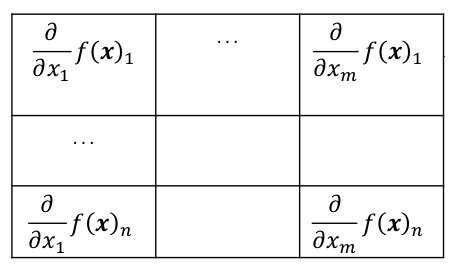
\includegraphics[width=7cm]{Images/jacobian.jpg}
    \caption{Jacobian Matrix}
\end{figure}

\noindent In Deep Learning the Jacobin matrix is used to update the computed minimum during the Gradient Descent algorithm.

\noindent Instead, the Hessian is a matrix of the second-order partial derivatives which describe the curvature of a multivariate function at a given point. It is the Jacobian of the gradient.

$$ f: \mathbb{R}^{n} \rightarrow \mathbb{R}, ~~ H \in \mathbb{R}^{n \times n} ~~~~ H_{ij} = \frac{\partial^2}{\partial x_i \partial x_j} f $$

\begin{figure}[h]
    \centering
    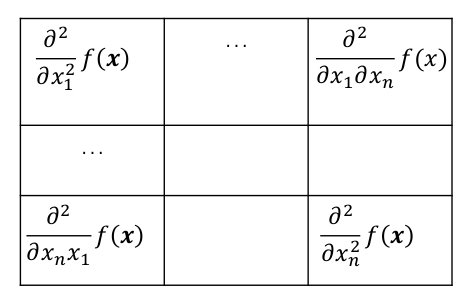
\includegraphics[width=7cm]{Images/hessian.jpg}
    \caption{Hessian Matrix}
\end{figure}

\noindent In the context of Deep Learning the Hessian is not very used as it is very expensive to compute. Nevertheless, second order methods have been proposed as an alternative to Gradient Descent. These ones have the advantage of knowing the direction in which the gradient is changing beforehand. This information can then be used to adjust the step size of the update rule making them converge more quickly and accurately to the local minimum than the Gradient Descent algorithm which operates only using first order derivatives.

\newpage
\subsection{Condition Number}

One application of the Hessian is computing the condition number. This is defined as a measure of the sensitivity of a function’s output to changes in its input and is calculated as the ratio of the maximum and minimum nonzero eigenvalues of the Hessian matrix.

$$ \left| \frac{ max(\lambda_i) }{min(\lambda_j)}  \right| $$


\noindent The condition number gives us information about the curvature in the different dimensions. A function with a high condition number indicates that the function has a large variation in its curvature, which can cause numerical instability, slow convergence and difficulty in finding the global minimum of the function. This is because in one direction the derivative increases rapidly, while in another direction it increases slowly. Therefore, the condition number can be used to diagnose if the the loss landscape is ill-conditioned which may lead to slow convergence or difficulties in optimization.


\begin{figure}[h]
    \centering
    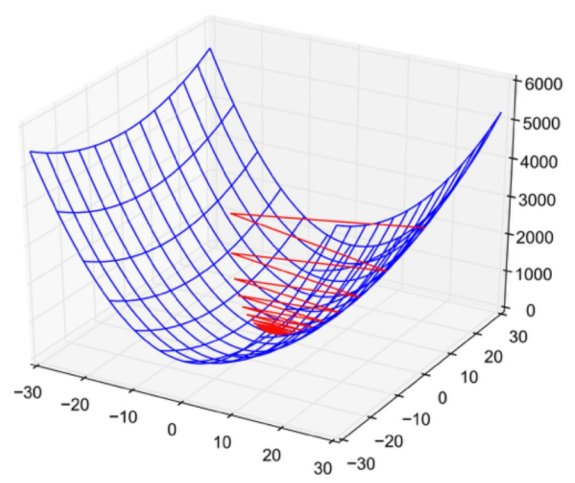
\includegraphics[width=7.5cm]{Images/condition_number.jpg}
    \caption{Condition Number}
    \label{fig:condition-number}
\end{figure}

\noindent In practise, the condition number is slow to compute since we need to calculate the Hessian beforehand. This is why is not so very used for Deep Learning. 